\beginsong{Papst und Sultan}[
    wuw={Christian Ludwig Noack}, 
    jahr={1789}, 
    bo={62}, 
    pfiii={68}, 
    kssiv={83}, 
    siru={95}, 
    tonspur={196}, 
    index={Der Papst lebt herrlich in der Welt},
]

\beginverse
\endverse
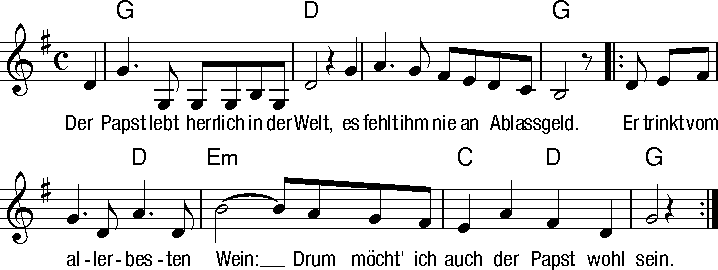
\includegraphics[draft=false, width=1\textwidth]{Noten/Lied075.pdf}	

\beginverse
\[G]Doch nein, er ist ein armer \[D]Wicht, ein holdes Mädchen küsst er \[G]nicht,
\lrep er schläft in seinem \[D]Bett al\[Em]lein: Drum möchte \[C]ich der \[D]Papst nicht \[G]sein. \rrep
\endverse

\beginverse
^Der Sultan lebt in Saus und ^Braus, er wohnt in einem Freuden^haus
\lrep voll wunderschöner ^Mägde^lein: Drum möcht' ich ^wohl der ^Sultan ^sein. \rrep
\endverse

\beginverse
^Doch nein, er ist ein armer ^Mann, denn folgt er seinem Alko^ran,
\lrep so trinkt er keinen ^Tropfen ^Wein: Drum möcht' ich ^auch nicht ^Sultan ^sein. \rrep
\endverse

\beginverse
^Geteilt veracht' ich beider ^Glück und kehr' in meinen Stand zu^rück,
\lrep doch das geh' ich mit ^Freuden ^ein: Halb Sultan ^und halb ^Papst zu ^sein. \rrep
\endverse

\beginverse
^Drum, Mädchen, gib mir einen ^Kuss, denn heut' bin ich dein Sulta^nus!
\lrep Ihr trauten Brüder, ^schenket ^ein, damit ich ^auch der ^Papst kann ^sein! \rrep
\endverse

\endsong
